\section{Querying Denormalized Data}

\subsection{Motivation}

\subsubsection{Where are we?}

An important component which is still missing from our discussion about storage and processing of denormalized data is the query language. With what we have covered, users are left with two options to handle denormalized data:
\begin{itemize}
    \item They can use an API within an imperative host language (e.g., Pandas in Python, or the MongoDB API in JavaScript, or the Spark RDD API in Java or Scala).
    \item Or they can push SQL, including ad-hoc extensions to support nestedness, to its limits.
\end{itemize}

APIs are unsatisfactory for complex analytics use cases. They are very convenient and suitable for Data Engineers that implement more data management layers on top of these APIs, but they are not suitable for end users who want to run queries to analyse data.

There is agreement in the database community that SQL is more satisfactory for the case that data is flat and homogeneous (relational tables).

SQL, possibly extended with a few dots, lateral view syntax and explode-like functions, will work nicely for the most simple use cases. But as soon as more complex functionality is needed, this approach becomes intractable. At best, this leads to gigantic and hard-to-read SQL queries. At worst, there is no way to express the use case in SQL. In both cases, the user ends up writing most of the code in an imperative language, invoking the lower-level API or nesting and chaining simple blocks of SQL.

In this chapter we will look at a query language called JSONiq which is tailor-made for denormalized data. It offers a data-independent layer on top of both data lakes and ETL-based, database management systems, similar to what SQL offers for (flat and homogeneous) relational tables.


\subsubsection{Denormalized Data}

\begin{figure}[h]
    \centering
    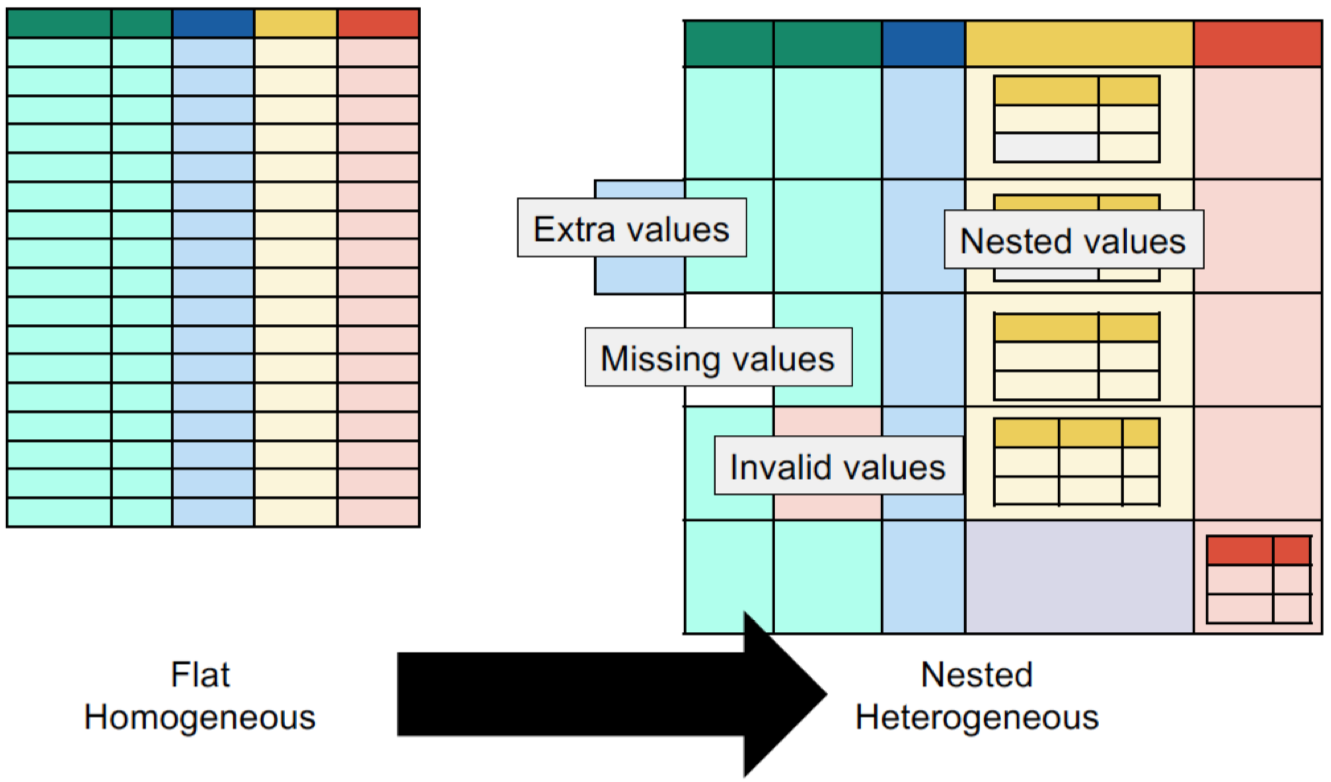
\includegraphics[width=0.7\textwidth]{Figures/DenormalizedData.png}
    \caption{Normalized vs. Denormalized Data}
\end{figure}

\subsubsection{Features of a Query Language}

A query language for datasets has three main features.

\paragraph{Declarative}
First, it is declarative. This means that the users do not focus on how the query is computed, but on what it should return. Thus, the database engine enjoys the flexibility to figure out the most efficient and fastest plan of execution to return the results.
(Python is imperative: do this, do that,... the user \underline{is} focused on how the query is computed.)

\paragraph{Functional}
Second, it is functional. This means that the query language is made of composable expressions that nest with each other, like a Lego game. Many, but not all, expressions can be seen as functions that take as input the output of their children expressions, and send their output to their parent expressions. However, the syntax of a good functional language should look nothing like a simple chain of function calls with parentheses and lambdas everywhere (this would then be an API, not a query language; examples of APIs are the Spark transformation APIs or Pandas): rather, expression syntax is carefully and naturally designed for ease of write and read. In complement to expressions, a rich function library (this time, with actual function call syntax) completes the expressions to a fully functional language.

\paragraph{Set-based}
Finally, it is set-based, in the sense that the values taken and returned by expressions are not only single values (scalars), but are large se- quences of items (in the case of SQL, an item is a row). In spite of the set-based terminology, set-based languages can still have bag or list semantics, in that they can allow for duplicates and sequences might be ordered on the logical level.


\subsubsection{JSONiq as a data calculator}

Here are some queries and their results.

\vspace{1\baselineskip}

\noindent
\begin{minipage}{0.16\textwidth}
\begin{center}
    \begin{tabular}{|c|c|}
        \hline
        Query & \texttt{1+1} \\ \hline
        Result & 2 \\ \hline
    \end{tabular}
\end{center}
\end{minipage}
\begin{minipage}{0.2\textwidth}
\begin{center}
    \begin{tabular}{|c|c|}
        \hline
        Query & \texttt{3+2*4} \\ \hline
        Result & 11 \\ \hline
    \end{tabular}
\end{center}
\end{minipage}
\begin{minipage}{0.2\textwidth}
\begin{center}
    \begin{tabular}{|c|c|}
        \hline
        Query & \texttt{2 < 5} \\ \hline
        Result & true \\ \hline
    \end{tabular}
\end{center}
\end{minipage}
\begin{minipage}{0.3\textwidth}
\begin{center}
    \begin{tabular}{|l|l|}
        \hline
        \multirow{2}{*}{Query} & \texttt{let \$i := 2} \\
         & \texttt{return \$i +1} \\ \hline
        Result & 3 \\ \hline
    \end{tabular}
\end{center}
\end{minipage}

\vspace{1\baselineskip}

\noindent
\begin{minipage}{0.2\textwidth}
\begin{center}
    \begin{tabular}{|c|c|}
        \hline
        Query & \texttt{[1,2,3]} \\ \hline
        Result & \texttt{[1,2,3]} \\ \hline
    \end{tabular}
\end{center}
\end{minipage}
\begin{minipage}{0.3\textwidth}
\begin{center}
    \begin{tabular}{|c|c|}
        \hline
        Query & \texttt{\{ "foo" : 1 \}} \\ \hline
        Result & \texttt{\{ "foo" : 1 \}} \\ \hline
    \end{tabular}
\end{center}
\end{minipage}
\begin{minipage}{0.3\textwidth}
\begin{center}
    \begin{tabular}{|c|c|}
        \hline
        Query & \texttt{\{ "foo" : 1 \}.foo} \\ \hline
        Result & \texttt{1} \\ \hline
    \end{tabular}
\end{center}
\end{minipage}

\vspace{1\baselineskip}

\noindent
\begin{minipage}{0.25\textwidth}
\begin{center}
    \begin{tabular}{|c|c|}
        \hline
        Query & \texttt{[1,2,3][[1]]} \\ \hline
        Result & \texttt{1} \\ \hline
    \end{tabular}
\end{center}
\end{minipage}
\begin{minipage}{0.5\textwidth}
\begin{center}
    \begin{tabular}{|c|c|}
        \hline
        Query & \texttt{\{ "foo" : [3,4,5] \}.foo[[1]] + 3} \\ \hline
        Result & \texttt{6} \\ \hline
    \end{tabular}
\end{center}
\end{minipage}

\vspace{1\baselineskip}

\noindent
\begin{minipage}{0.4\textwidth}
\begin{center}
    \begin{tabular}{|c|c|}
        \hline
        Query & \texttt{\{ "foo" : [3,4,5] \}.foo[]} \\ \hline
        \multirow{3}{*}{Result} & \texttt{3} \\
         & \texttt{4} \\
         & \texttt{5} \\ \hline
    \end{tabular}
\end{center}
\end{minipage}
\begin{minipage}{0.2\textwidth}
\begin{center}
    \begin{tabular}{|c|c|}
        \hline
        Query & \texttt{1 to 4} \\ \hline
        \multirow{4}{*}{Result} & \texttt{1} \\
            & \texttt{2} \\
            & \texttt{3} \\
            & \texttt{4} \\ \hline
    \end{tabular}
\end{center}
\end{minipage}
\begin{minipage}{0.4\textwidth}
\begin{center}
    \begin{tabular}{|l|l|}
        \hline
        \multirow{2}{*}{Query} & \texttt{for \$i in 3 to 5} \\
         & \texttt{return \{ \$i : \$i * \$i \} } \\ \hline
        \multirow{3}{*}{Result} & \texttt{9} \\
            & \texttt{16} \\
            & \texttt{25} \\ \hline
    \end{tabular}
\end{center}
\end{minipage}

\vspace{1\baselineskip}

\noindent
\begin{minipage}{0.66\textwidth}
\begin{center}
    \begin{tabular}{|l|l|}
        \hline
        \multirow{4}{*}{Query} & \texttt{keys(} \\
            & \texttt{  for \$i in json-file("s3://bucket/myfiles/json/*")} \\
            & \texttt{  return \$i} \\
            & \texttt{)} \\ \hline
        \multirow{2}{*}{Result} & \texttt{"foo"} \\
            & \texttt{"bar"} \\ \hline
    \end{tabular}
\end{center}
\end{minipage}

\vspace{1\baselineskip}

\noindent
\begin{minipage}{0.72\textwidth}
\begin{center}
    \begin{tabular}{|l|l|}
        \hline
        \multirow{6}{*}{Query} & \texttt{keys(} \\
            & \texttt{  for \$i in parquet-file( "s3://bucket/myfiles/parquet" )} \\
            & \texttt{  return \$i} \\
            & \texttt{)} \\ \hline
        \multirow{2}{*}{Result} & \texttt{"foo"} \\
            & \texttt{"bar"} \\ \hline
    \end{tabular}
\end{center}
\end{minipage}


\subsection{The JSONiq Data Model}

Every expression of the JSONiq "data calculator" returns a sequence of items. Always. An item can be either an object, an array, an atomic item, or a function item.
Atomic items can be any of the "core" JSON types: strings, numbers (integers, decimals, doubles...), booleans and nulls, but JSONiq has a much richer type system. You can also have Objects (\texttt{\{"foo" : "bar"\}}) and Arrays (\texttt{$[$"foo","bar"$]$}).

Sequences of items are flat, in that sequences cannot be nested. But they scale massively and can contain billions or trillions of items. The only way to nest lists is to use arrays (which can be recursively nested). Sequences can be homogeneous or heterogeneous. One item is logically the same as a sequence of one item. A sequence can also be empty. Caution, the empty sequence is not the same logically as a null item.

\begin{figure}[h]
    \centering
    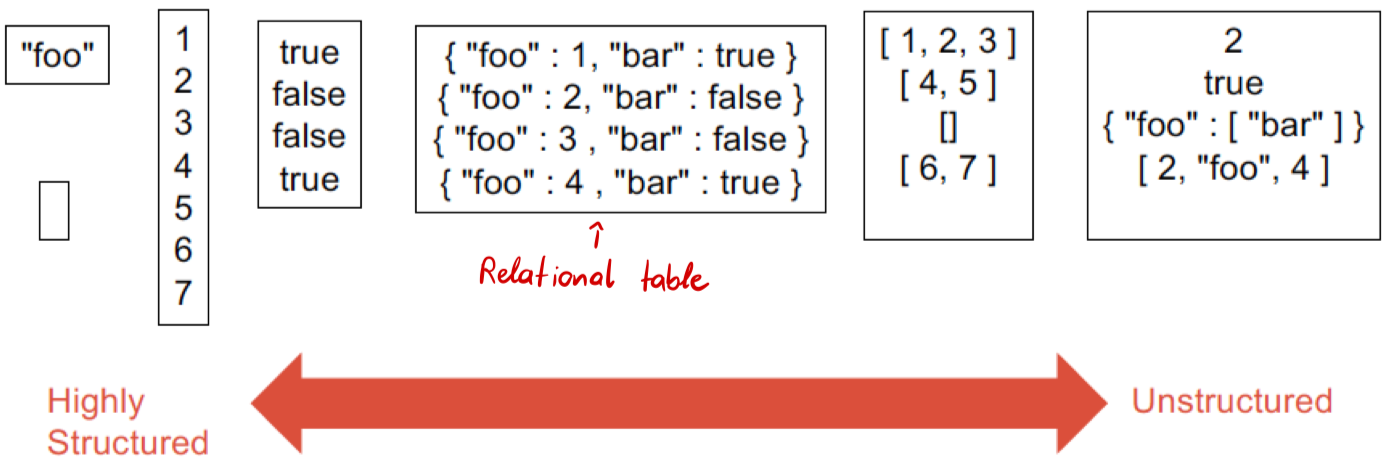
\includegraphics[width=0.7\textwidth]{Figures/SequenceofItems.png}
    \caption{Sequences of Items}
\end{figure}

\subsection{Navigation}

Assume we have a JSON document with the name file.json and the following content:
\begin{lstlisting}[style=json]
{
    "o" : [
        { "a" : {
                "b" : [
                    { "c" : 1, "d" : "a" }
                ]
            }
        },
        { "a" : {
                "b" : [
                    { "c" : 1, "d" : "f" },
                    { "c" : 2, "d" : "b" }
                ]
            }
        },
        ...,
        { "a" : {
                "b" : [
                  { "c" : 3, "d" : "l" },
                  { "c" : 1, "d" : "m" },
                  { "c" : 0, "d" : "k" }
                ]
            }
        }
    ]
}
\end{lstlisting}

\paragraph{Open File}
We can open this document and return its content with \texttt{json-doc("file.json")}. The return is the same as the whole file.

\paragraph{Object Lookups}
It is possible to navigate into objets with dots, similar to object-oriented programming. For example \texttt{json-doc("file.json").o} returns the value associated with the key \texttt{o}. This returned an array, more precisely, a sequence of one array item.

\paragraph{Array Unboxing}
We can unbox the array, meaning, extract its members as a sequence of object items, with empty square brackets, like so: \texttt{json-doc("file.json").o[]}

\paragraph{Parallel Navigation}
The dot syntax, in fact, works on sequences, too. It will extract the value associated with a key in every object of the sequence (anything else than an object is ignored and thrown away):

\begin{lstlisting}[style=json]
// Query:
json-doc("file.json").o[].a

// Result:
{ "b" : [ { "c" : 1, "d" : "a" }]}
{ "b" : [ { "c" : 1, "d" : "f" },
          { "c" : 2, "d" : "b" } ] }
{ "b" : [ { "c" : 4, "d" : "e" },
          { "c" : 8, "d" : "d" },
          { "c" : 3, "d" : "c" } ] }
{ "b" : [ ] }
{ "b" : [ { "c" : 3, "d" : "h" } ] }
{ "b" : [ { "c" : 4, "d" : "g" } ] }
{ "b" : [ { "c" : 3, "d" : "l" } ] }
\end{lstlisting}

Array unboxing works on sequences, too. Note how all the members are concatenated to a single, merged sequence, similar to a flatMap in Apache Spark.

\begin{lstlisting}[style=json]
// Query:
json-doc("file.json").o[].a.b[]

// Result:
{ "c" : 1, "d" : "a" }
{ "c" : 1, "d" : "f" }
{ "c" : 2, "d" : "b" }
{ "c" : 4, "d" : "e" }
{ "c" : 8, "d" : "d" }
{ "c" : 3, "d" : "c" }
{ "c" : 3, "d" : "h" }
{ "c" : 4, "d" : "g" }
{ "c" : 3, "d" : "l" }
\end{lstlisting}

\paragraph{Filtering with predicates}
It is possible to filter any sequence with a predicate, where \$\$ in the predicate refers to the current item being tested.

\begin{lstlisting}[style=json]
// Query:
json-doc("file.json").o[].a.b[][$$.c = 3]

// Result:
{ "c" : 3, "d" : "c" }
{ "c" : 3, "d" : "h" }
{ "c" : 3, "d" : "l" }
\end{lstlisting}

It is also possible to access the item at position n in a sequence with this same notation: if what is inside the square brackets is a Boolean, then it acts as a filtering predicate; if it is an integer, it acts as a position (we start counting at 1):

\begin{lstlisting}[style=json]
// Query:
json-doc("file.json").o[].a.b[][5]

// Result:
{ "c" : 8, "d" : "d" }
\end{lstlisting}

\paragraph{Array Lookup}
To access the n-th member of an array, you can use double-squarebrackets, like so:

\begin{lstlisting}[style=json]
// Query:
json-doc("file.json").o[[2]].a

// Result:
{"b":[{ "c" : 1, "d" : "f" },
      { "c" : 2, "d" : "b" } ] }
\end{lstlisting}

Like dot object navigation and unboxing, double square brackets (array navigation) work with sequences as well. For any array that has less elements than the requested position, as well as for items that are not arrays, no items are contributed to the output:

\begin{lstlisting}[style=json]
// Query:
json-doc("file.json").o[].a.b[[2]]

// Result:
{ "c" : 2, "d" : "b" }
{ "c" : 8, "d" : "d" }
\end{lstlisting}

\paragraph{A common pitfall: Array lookup vs. Sequence predicates}
Do not confuse sequence positions (single square brackets) with array positions (double square brackets)! The difference is easy to see on a simple example involving a sequence of two arrays with two members each:

\begin{lstlisting}[style=json]
// Query:
([1,2],[3,4])[2]
// Result:
[3,4]

// Query:
([1,2],[3,4])[[2]]
// Result:
2
4
\end{lstlisting}


\subsection{Schema Discovery}

\paragraph{Collections}
Many datasets are in fact found in the form of large collections of smaller objects. Such collections are accessed with a function call together with a name or (if reading from a data lake) a path. The name of the function can vary and in this Chapter we will just use the W3C-standard collection function. In RumbleDB, a JSON Lines dataset is accessed with the function json-line, in a similar way.

\begin{lstlisting}[style=json]
// Query:
collection( "https://www.rumbledb.org/samples/git-archive.jsonl" )

// Result:
{ "id" : "7045118886", "type" : "PushEvent", ...
{ "id" : "7045118891", "type" : "PushEvent", ...
{ "id" : "7045118892", "type" : "PullRequestEvent", ...
...
\end{lstlisting}

You can also at the first element of the collection or at the top N objects using the position function in a predicate, which returns the position in the sequence of the current item being tested by the predicate (similar to the LIMIT clause in SQL):

\begin{lstlisting}[style=json]
// Query:
collection( "https://www.rumbledb.org/samples/git-archive.jsonl" )[1]

// Result:
{ "id" : "7045118886", "type" : "PushEvent", ...

// Query:
collection( "https://www.rumbledb.org/samples/git-archive.jsonl" )[position() le 3]

// Result:
{ "id" : "7045118886", "type" : "PushEvent", ...
{ "id" : "7045118891", "type" : "PushEvent", ...
{ "id" : "7045118892", "type" : "PullRequestEvent", ...
\end{lstlisting}

\paragraph{Getting all top-level keys}
The keys function retrieves all keys. It can be called on the entire sequence of objects and will return all unique keys found (at the top level) in that collection:

\begin{lstlisting}[style=json]
// Query:
keys(collection( "https://www.rumbledb.org/samples/git-archive.jsonl" ))

// Result:
"repo"
"org"
"actor"
"public"
"type"
"created_at"
"id"
"payload"
\end{lstlisting}

\paragraph{Getting unique values associated with a key}
With dot object lookup, we can look at all the values associated with a key like so:

\begin{lstlisting}[style=json]
// Query:
collection( "https://www.rumbledb.org/samples/git-archive.jsonl" ).type

// Result:
"PushEvent"
"PushEvent"
"PullRequestEvent"
"PushEvent"
...
\end{lstlisting}

With distinct-values, it is then possible to eliminate duplicates and look at unique values:

\begin{lstlisting}[style=json]
// Query
distinct-values(collection( "https://www.rumbledb.org/samples/git-archive.jsonl" ).type)

// Result:
"PullRequestEvent"
"MemberEvent"
"PushEvent"
"IssuesEvent"
"PublicEvent"
...
\end{lstlisting}

\paragraph{Aggregations}
Aggregations can be made on entire sequences with a single function call. The five basic functions are count, sum, avg, min, max. Obvi- ously, the last four require numeric values and will otherwise throw an error.

\begin{lstlisting}[style=json]
// Query:
count(distinct-values(collection( "https://www.rumbledb.org/samples/git-archive.jsonl" ).type))

// Result:
3597

// Query:
count(collection( "https://www.rumbledb.org/samples/git-archive.jsonl" ))

// Result:
36577
\end{lstlisting}


\subsection{Construction}

\paragraph{Construction of atomic values}

Since it is a declarative language, you can just write them down. Atomic values that are core to JSON can be constructed with exactly the same syntax as JSON. E.g.

\begin{lstlisting}[style=json]
// Query:
"foo"

// Result:
"foo"
\end{lstlisting}

For more specific types, a cast is needed. This works with any of the atomic types. There are two syntaxes for this:

\begin{lstlisting}[style=json]
// Query:
NonNegativeInteger("42")
// or:
"42" cast as NonNegativeInteger

// Result:
42

// Other examples:
date("2013-05-01Z")
dateTimeStamp("2013-06-21-T05:00:00Z")
hexBinary("0CD7")
...
\end{lstlisting}

\paragraph{Construction of objects and arrays}
Objects and arrays are constructed with the same syntax as JSON. In fact, one can copy-paste any JSON value, and it will always be recognized as a valid JSONiq query returning that value.

\paragraph{Construction of sequences}
Sequences can be constructed (and concatenated) using commas:

\begin{lstlisting}[style=json]
// Query:
[2,3],true,"foo",{"f":1}

// Result:
[2,3]
true
"foo"
{"f":1}
\end{lstlisting}

Increasing sequences of integers can also be built with the to key-word: \texttt{1 to 100}.


\subsection{Scalar Expressions}
JSONiq supports basic arithmetic: addition (+), subtraction (-), multiplication (*), division (not a slash, but \texttt{div}), integer division (idiv) and modulo (mod). If both sides have exactly one item, the semantics is relatively natural.

If one side is a double and the other is a float or a decimal, a double is returned. If one side is a float and the other is a decimal, then a float is returned. If one side is a decimal and the other an integer, a decimal is returned.

If one side (or both) is the empty sequence, then the arithmetic expression returns an empty sequence without an error. If one of the two sides is null (and the other side is not the empty sequence), then the arithmetic expression returns null. If one of the sides (or both) is not a number, null, or the empty sequence, then a type error is thrown (for example when one side is a string). However, if the left side is a date and the right is a duration, you cann add the two to obtain a new date.

\paragraph{String Manipulation}
You can concatenate strings in different ways:
\begin{lstlisting}[style=json]
// Queries:
"foo" || "bar"
concat("foo","bar")
// Result:
"foobar"

// Query:
string-join(("foo","bar","foobar"),"-")
// Result:
"foo-bar-foobar"

// Query:
substr("foobar",4,3)
// Result:
"bar"

// Query:
string-length("foobar")
// Result:
6
\end{lstlisting}

\paragraph{Value Comparison}
Sequences of one atomic item can be compared.
\begin{lstlisting}[style=json]
// Queries:
1+1 eq 2
1+1 = 2
// Result
true

// Query:
6*7 ne 21*2
6*7 != 21*2
// Result:
false

// Query:
234 gt 123
// Result:
true

// Query:
null le 2
// Result:
null
\end{lstlisting}

If one of the two sides is the empty sequence, then the value com- parison expression returns an empty sequence as well.

You cannot compare strings with integers, that will through an error (but MongoDB won't).


\paragraph{General Comparison}
Comparison also works on sequences. When you try to apply a comparison to a sequence, it tries to find a match on both sides. It will return true if it finds an item in the sequence on the left matching the value on the right, that fulfil the criteria. It basically applies an existential quantification ("it exists" on the left and on the right.)
\begin{lstlisting}[style=json]
// Query:
(1,2,3,4,5) = 1
// Result:
true

// Query:
(1,2,3,4,5) < (2,3,4,5,6)
// Result
true

// Query
(1,2,3,4,5) >= (6,7,8,9,10)
// Result
false
\end{lstlisting}
The second example is true because it compares it elementwise. So because $1$ is smaller then for example $3$, it will already return true. In the third example there is no element in the left sequence larger than any of the elements in the right sequence, thus it will return false.

You will get an error if one of the elements in the sequence is a string. Furthermore, you will always get \texttt{false} if you apply a comparison ot an empty sequence. Think about it as "the empty sequence is, well, empty, and thus there cannot exist any element matching (or greater than or ...) any of the elements in the other sequence on the other side of the comparison".

\paragraph{Logic}
JSONiq supports the three basic logic expressions and, or, and not. not has the highest precedence, then and, then or.

\begin{lstlisting}[style=json]
// Query:
1+1 eq 2 and (2+2 eq 4 or not 100 mod 5 eq 0)
// Result:
true

// Query:
every $i in 1 to 10
satisfies $i gt 0
// Result:
true

// Query:
some $i in 1 to 10
satisfies $i gt 5
// Result:
true
\end{lstlisting}


\subsection{Composablility}
JSONiq, as a functional language, is modular. This means that expressions can be combined at will, exactly like one would combine addition, multiplication, etc, at will. At least as long as the types of the ouputs and inputs are compatible.

You can also have functions inside json objects:
\begin{lstlisting}[style=json]
// Query:
{
    "attr" : string-length("foobar")
    "values" : [
        for $i in 1 to 10
        return long($i)
    ]
}
// Result:
{
    "attr" : 6
    "values" : [ 1, 2, 3, 4, 5, 6, 7, 8, 9, 10 ]
}
\end{lstlisting}

Precedence (low first):
\begin{itemize}
    \item Comma
    \item Data Flow (FLWOR, if-then-else, switch...)
    \item Logic
    \item Comparison
    \item String concatenation
    \item Range
    \item Arithmetic
    \item Path expression
    \item Filter predicates, dynamic function calls
    \item Literals, constructors and variables
    \item Function calls, named function references, inline functions
\end{itemize}

Precedence can be easily overridden with parentheses. This is often useful when one does not know the precedence ordering by heart.


\subsubsection{Data Flow}

\paragraph{if-then-else}
In an if-then-else statement, you have a condition and the actions for if the statement is true or false.

\begin{lstlisting}[style=json]
// Query:
if(count(json-file("file.json").o) gt 1000)
then "Large file!"
else "Small file."
// Result:
"Small file."
\end{lstlisting}

\paragraph{Switch}
The expression inside the swich is evaluated and an error is thrown if more than one item is returned. Then, the resulting item is compared for equality with each one of the candidate values. The result of the expression corresponding to the first match is taken, and if there are no matches, the result of the default expression is taken.

\begin{lstlisting}[style=json]
// Query:
switch(json-file("file.json").o[[1]].a.b[[1]].c)
case 1 return "one"
case 2 return "two"
default return "other"
// Result:
"one"
\end{lstlisting}

\paragraph{Try-Catch}
If the expression in the try clause is successfully evaluated, then its results are taken. If there is an error, then the results of the expression in the first catch clause matching the error is taken (* being the joker).

\begin{lstlisting}[style=json]
// Query:
try {
    date(json-file("file.json").o[[1]].a.b[[1]].c)
} catch * {
    "This is not a date!"
}
// Result:
"This is not a date!"
\end{lstlisting}


\subsection{Binding Variables with Cascades of let Clauses}
The following two queries are equivalent:

\begin{lstlisting}[style=json]
// Query 1:
json-doc("file.json").o[].a.b[].c = 1
// Query 2:
let $a := json-doc("file.json")
let $b := $a.o
let $c := $b[]
let $d := $c.a
let $e : $d.b
let $f := $d[]
let $g := $f.c
return $g = 1
// Result:
true
\end{lstlisting}

Variables in JSONiq start with a dollar sign. This way of subsequently binding variables to compute intermediate results is typical of functional language.
It is important to understand that this is not a variable assignment that would change the value of a variable. This is only a declarative binding.

\subsection{FLWOR Expressions}

One of the most important and powerful features of JSONiq is the FLWOR (for, let, where, order-by, return) expression. It corresponds to SELECT-FROM-WHERE queries in SQL, however, it is considerably more expressive and generic than them in several aspects:
\begin{itemize}
    \item In SQL, the clauses must appear in a specific order (SELECT, FROM, WHERE, GROUB BY, HAVING, ORDER BY, OFFSET, LIMIT) whereas in JSONiq, clauses can appear in any order except for the first and the last one.
    \item JSONiq supports a let clause, which does not exist in SQL. Let clauses make it very convenient to write and organize more com- plex queries.
    \item In SQL, when iterating over multiple tables in the FROM clause, they “do not see each other”, i.e., the semantics is (logically) that of a Cartesian product. In JSONiq, for clauses (which correspond to FROM clauses in SQL), do see each other, meaning that it is possible to iterate in higher and higher levels of nesting by referring to a previous for variable. This is both easier to write and read than lateral views, and it is also more expressive.
    \item The semantics of FLWOR clauses is simple, clean, and inherently functional; it is based on tuple streams containing variable bindings, which flow from clause to clause. There is no “spooky action at a distance” such as the explode() function, which indirectly causes a duplication of rows in Spark SQL.
\end{itemize}

\subsubsection{Simple Dataset}
We will work with the following datasets:

\begin{lstlisting}[style=json]
// products.json
{"pid":1, "type" : "tv", "store":1}
{"pid":2, "type" : "tv", "store":2}
{"pid":3, "type" : "phone", "store":2}
{"pid":4, "type" : "tv", "store":3}
{"pid":5, "type" : "teapot", "store":2}
{"pid":6, "type" : "tv", "store":1}
{"pid":7, "type" : "teapot", "store":2}
{"pid":8, "type" : "phone", "store":4}

// stores.json
{ "sid" : 1, "country" : "Switzerland" }
{ "sid" : 2, "country" : "Germany" }
{ "sid" : 3, "country" : "United States" }
\end{lstlisting}

\subsubsection{For Clauses}
A few examples:
\begin{lstlisting}[style=json]
// Query:
for $x in 1 to 3
return { "number": $x, "square": $x * $x }
// Result
{ "number" : 1, "square" : 1 }
{ "number" : 2, "square" : 4 }
{ "number" : 3, "square" : 9 }

// Query
for $product in json-file("products.json")
return project($product, ("type", "store"))
// Result
{"type" : "tv", "store":1}
{"type" : "tv", "store":2}
{"type" : "phone", "store":2}
...

// Query
for $product in json-file("products.json")
for $store in json-file("stores.json")[$$.sid eq $product.store]
return { "product" : $product.type, "country" : $store.country }
// Result
{"product" : "tv", "country":"Switzerland"}
{"product" : "tv", "country":"Germany"}
{"product" : "phone", "country":"Germany"}
...
\end{lstlisting}

\subsubsection{Let Clauses}
A few examples:
\begin{lstlisting}[style=json]
// Query:
for $x in 1 to 10
let $square-and-cube := ($x * $x, $x * $x * $x)
return{
    "number": $x,
    "square": $square-and-cube[1],
    "cube": $square-and-cube[2]
}
// Result:
{ "number" : 1, "square" : 1, "cube" : 1 }
{ "number" : 2, "square" : 4, "cube" : 8 }
{ "number" : 3, "square" : 9, "cube" : 27 }
{ "number" : 4, "square" : 16, "cube" : 64 }
{ "number" : 5, "square" : 25, "cube" : 125 }
{ "number" : 6, "square" : 36, "cube" : 216 }
{ "number" : 7, "square" : 49, "cube" : 343 }
{ "number" : 8, "square" : 64, "cube" : 512 }
{ "number" : 9, "square" : 81, "cube" : 729 }
{ "number" : 10, "square" : 100, "cube" : 1000 }

// Query:
for $store in json-file("stores.json")
let $product := json-file("products.json")[$store.sid eq $$.store]
return {
  "store" : $store.country,
  "available products" : [
    distinct-values($product.type)
  ]
}
// Result:
{
 "store" : "Germany",
 "available products" : [
    "tv",
    "teapot",
    "phone" ]
}
{
 "store" : "Switzerland",
 "available products" : [ "tv" ]
}
{
 "store" : "United States",
 "available products" : [ "tv" ]
}
\end{lstlisting}


\subsubsection{Where Clauses}
Where clauses are used to filter variable bindings (tuples) based on a predicate on these variables. They are the equivalent to a WHERE clause in SQL. A where clause can appear anywhere in a FLWOR expression, except that it cannot be the first clause (always for or let) or the last clause (always return).

A where clause always outputs a subset (or all) of its incoming tuples, without any alteration. In the case that the predicate always evaluates to true, it forwards all tuples, as if there had been no where clause at all. In the case that the predicate always evaluates to false, it outputs no tuple and the FLWOR expression will then return the empty sequence, with no need to further evaluate any of the remaining clauses.

An example:

\begin{lstlisting}[style=json]
// Query
for $product in json-file("products.json")
let $store := json-file("stores.json")[$$.sid eq $product.store]
where $store.country = "Germany"
return $product.type
// Result
"tv"
"phone"
"teapot"
"teapot"
\end{lstlisting}

\subsubsection{Order by Clauses}
Order by clauses are used to reorganize the order of the tuples, but without altering them. In case of ties between tuples, the order is arbitrary. But it is possible to sort on another variable in case there is a tie with the first one (compound sorting keys).
A few examples:

\begin{lstlisting}[style=json]
// Query:
for $x in -2 to 2
let $square := $x * $x
order by $square descending, $x ascending
return {
  "number": $x,
  "square": $square
}
// Result:
{ "number" : -2, "square" : 4 }
{ "number" : 2, "square" : 4 }
{ "number" : -1, "square" : 1 }
{ "number" : 1, "square" : 1 }
{ "number" : 0, "square" : 0 }

// Query:
for $product in json-file("products.json")
let $store := json-file("stores.json")[$$.sid eq $product.store]
group by $t := $product.type
order by count($store) descending, string-length($t) ascending
return $t
// Result:
"tv"
"teapot"
"phone"
\end{lstlisting}

\subsubsection{Groub by Clauses}
Group by clauses organize tuples in groups based on matching keys, and then output only one tuple for each group, aggregating other variables.
However, JSONiq's group by clauses are more powerful and expres- sive than SQL GROUP BY clauses: indeed, it is also possible to opt out of aggregating other (non-grouping-key) variables. Then, for a non-aggregated variable, the sequence of all its values within a group will be rebound to this same variable as a single binding in the outcoming tuple. It is thus possible to write many more queries than SQL would allow, which is one of the reasons why a language like JSONiq should be preferred for nested datasets.
A few examples:

\begin{lstlisting}[style=json]
// Query:
for $x in 1 to 5
let $y := $x mod 2
group by $y
return {
    "grouping key" : $y,
    "grouped x values" : [ $x ],
}
// Result:
{
    "grouping key" : 0,
    "grouped x values" : [ 2, 4 ]
}
{
    "grouping key" : 1,
    "grouped x values" : [ 1, 3, 5 ]
}

// Query:
for $product in json-file("products.json")
group by $sid := $product.sid
order by $sid
let $store := json-file("stores.json")
                [$$.sid = $sid]
return {|
  $store,
  { "products" : [ distinct-values($product.type) ] }
|}
// Result:
{
    "sid" : 1,
    "country" : "Switzerland",
    "products"  [ "tv" ]
}
{
    "sid" : 2,
    "country" : "Germany",
    "products" : [ "tv", "phone", "teapot" ]
}
{
    "sid" : 3,
    "country" : "United States",
    "products" : [ "tv" ]
}
\end{lstlisting}

\subsubsection{Tuple Stream Vizualization}

An illustration can be seen in \cref{fig:TupleStream}.
Note that these tuple streams are not sequences of items, because clauses are not expressions; tuple streams are only a formal description of the semantics of FLWOR expressions and their visual- ization as DataFrames is pedagogical. Having said that, the reader may have guessed that tuple streams can be internally implemented as Spark DataFrames, and in fact, RumbleDB does just that (but it hides it from the user).

\begin{figure}[H]
    \centering
    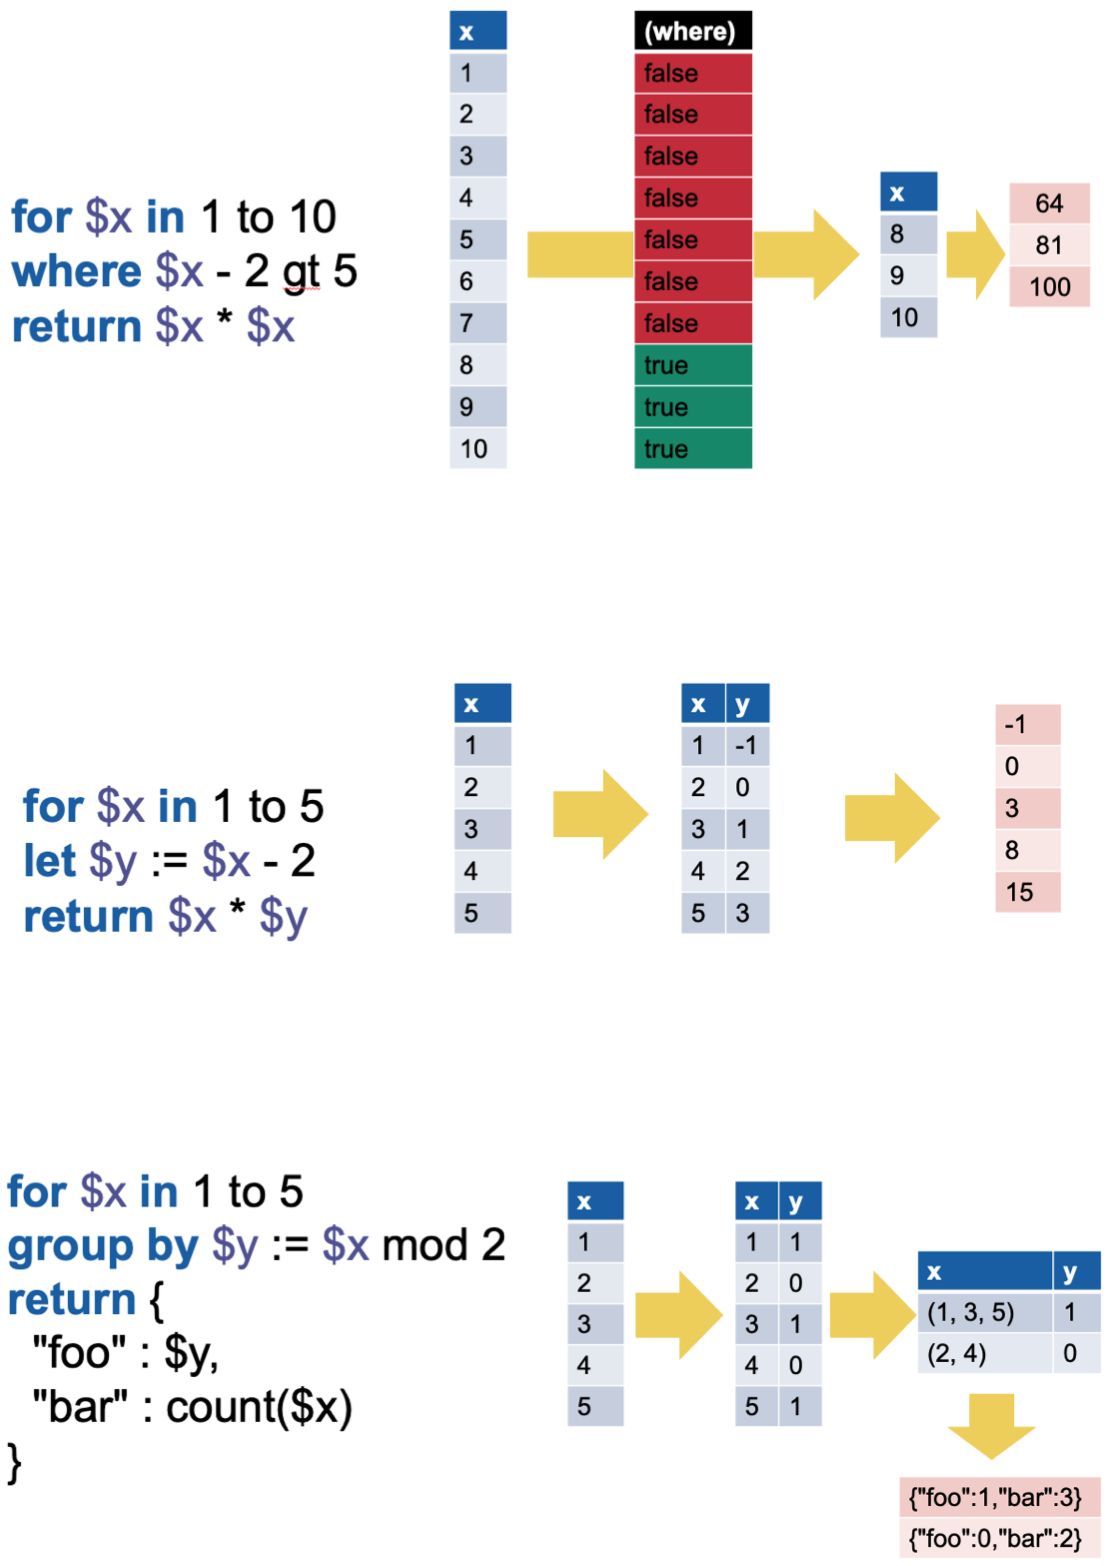
\includegraphics[width=0.5\textwidth]{Figures/TupleStream.png}
    \caption{Tuple Stream Vizualization}\label{fig:TupleStream}
\end{figure}


\subsubsection{Relational Algebra with JSONiq}
Assume we are dealing again with the following dataset:

\begin{lstlisting}[style=json]
// products.json
{"id":1, "type" : "tv", "store":1}
{"id":2, "type" : "tv", "store":2}
{"id":3, "type" : "phone", "store":2}
{"id":4, "type" : "tv", "store":3}
{"id":5, "type" : "teapot", "store":2}
{"id":6, "type" : "tv", "store":1}
{"id":7, "type" : "teapot", "store":2}
{"id":8, "type" : "phone", "store":4}

// stores.json
{ "id" : 1, "country" : "Switzerland" }
{ "id" : 2, "country" : "Germany" }
{ "id" : 3, "country" : "United States" }
\end{lstlisting}

\paragraph{Selection}
Example:
\begin{lstlisting}[style=json]
// Query:
for $p in json-file("products.json")
where $p.store = "1"
return $p
// Result:
{"id":1, "type" : "tv", "store":1}
{"id":6, "type" : "tv", "store":1}
\end{lstlisting}

\paragraph{Projection}
Example:
\begin{lstlisting}[style=json]
// Query:
for $p$ in json-file("products.json")
return project($p,("id","type"))
// Result:
{"id" : 1, "type" : "tv"}
{"id":2, "type" : "tv"}
{"id":3, "type" : "phone"}
...
\end{lstlisting}

\paragraph{Ordering}
Example:
\begin{lstlisting}[style=json]
// Query:
for $p$ in json-file("products.json")
order by $p.id
return $p
// Result:
{"id":1, "type" : "tv", "store":1}
{"id":2, "type" : "tv", "store":2}
{"id":3, "type" : "phone", "store":2}
...
\end{lstlisting}

\paragraph{Aggregation}
Example:
\begin{lstlisting}[style=json]
// Query:
for $p$ in json-file("products.json")
group by $t := $p.type
return {
    "type" : $t,
    "num" : count($p)
}
// Result:
{"type" : "tv", "num" : 4}
{"type" : "phone", "num" : 1}
{"type" : "teapot", "num" : 2}
\end{lstlisting}

\paragraph{Join}
RumbleDB auto-detects joins and it will implement it on top of Spark as actual joins.
Example:
\begin{lstlisting}[style=json]
// Query:
for $p in json-file("products.json")
for $s in json-file("stores.json")
where $p.store eq $s.id
return{
    "type" : $p.type,
    "country" : $s.country
}
// Result:
{"type" : "tv", "country" : "Switzerland"}
{"type" : "tv", "country" : "Germany"}
{"type" : "phone", "country" : "Germany"}
...
{"type" : "teapot", "country" : "Germany"}
\end{lstlisting}

\paragraph{Left-outer Join}
A special case of join where not everything has a match. You can implement that with the \texttt{allowing empty in} command. It will return \texttt{null} for empty items.
Example:
\begin{lstlisting}[style=json]
// Query:
for $p in json-file("products.json")
for $s allowing empty in
    json-file("store.json")[$p.store eq $$.id]
return {
    "type" : $p.type,
    "country" : $s.country
}
// Result:
{"type" : "tv", "country" : "Switzerland"}
{"type" : "tv", "country" : "Germany"}
...
{"type" : "teapot", "country" : "Germany"}
{"type" : "foo", "country" : null}
\end{lstlisting}

\paragraph{Denormalization}
This is something SQL cannot do. In the following example \texttt{\$\$} is the \textit{context item}. It is bound one-to-one to the items of the sequence it is refered to.

\begin{lstlisting}[style=json]
// Query:
for $s in json-file("stores.json")
let $p:= json-file("products.json")[$$.store eq $s.id]
return{
    "country" : $s.country,
    "products" : [$p.type]
}
// Result:
{"country" : "Switzerland", "products" : ["tv","tv"]}
{"country" : "Germany", "products" : ["tv","phone","teapot","teapot"]}
{"country" : "United States", "products" : ["tv"]}
\end{lstlisting}

\subsection{Types}

\subsubsection{Variable Types}
It is possible to annotate any FLWOR variable with an expected type as shown below.

\begin{lstlisting}[style=json]
let $path as string := "git-archive-big.json"
let $events as object* := json-file($path)
let $actors as object* := $events.actor
let $logins as string* := $actors.login
let $distinct-logins as string* := distinct-values($logins)
let $count as integer := count($distinct-logins)
return $count
\end{lstlisting}

Since every value in JSONiq is a sequence of item, a sequence type consists of two parts: an item type, and a cardinality.
Item types can be any of the builtin atomic types (JSound), as well as “object”, “array” and the most generic item type, “item”. Cardinality can be one of the following four:
\begin{itemize}
    \item Any number of items (suffix *), e.g. object*
    \item One or more items (suffix +), e.g. array+
    \item Zero or one item (suffix ?), e.g. boolean?
    \item Exactly one item (no suffix), e.g. integer
\end{itemize}
If it is detected, at runtime, that a sequence of items is bound to a variable but does not match the expected sequence type, either because one of the items does not match the expected item type, or because the cardinality of the sequence does not match the expected cardinality, then a type error is thrown and the query is not evaluated.
It is also possible to annotate variables in for clauses, however the cardinality of the sequence type of a for variable will logically be either one (no suffix), or zero-or-one (?) in the case that “allowing empty” is specified.

\subsubsection{Type Expressions}
JSONiq has a few expressions related to types.

An \texttt{instance of} expression checks whether a sequences matches a
sequence type, and returns true or false. This is similar to the homony- mous expression in Java.

\begin{lstlisting}[style=json]
// Query:
(3.14, "foo") instance of integer*,
([1], [ 2, 3 ]) instance of array+
// Result:
false
true  
\end{lstlisting}

A \texttt{cast as} expression casts single items to an expected item type.

\begin{lstlisting}[style=json]
// Query:
"3.14" cast as decimal
// Result:
3.14
\end{lstlisting}

A \texttt{castable as} expression tests whether a cast would succeed (in which case it returns true) or not (false).

\begin{lstlisting}[style=json]
// Query:
"3.14" castable as decimal
// Result:
true
\end{lstlisting}

A \texttt{treat as} expression checks whether its input sequence matches an expected type (like a type on a variable); if it does, the input sequence is returned unchanged. If not, an error is raised. This is useful in complex queries and for debugging purposes.

\begin{lstlisting}[style=json]
// Query:
[ 1, 2, 3, 4][] treat as integer+
// Result:
1
2
3
4
\end{lstlisting}

\subsubsection{Types in User-defined Functions}
JSONiq supports user-defined functions. Parameter types can be optionally specified, and a return type can also be optionally specified. The following two queries have the same result:

\begin{lstlisting}[style=json]
// Query 1:
declare function is-big-data(
    $threshold as integer,
    $objects as object*
) as boolean
{
    count($objects) gt $threshold
};

is-big-data(1000, json-file("git-archive.json"))

// Query 2:
declare function is-big-data(
    $threshold,
    $objects
)
{
    count($objects) gt $threshold
};

is-big-data(1000, json-file("git-archive.json"))

// Result:
true
\end{lstlisting}

\subsubsection{Validating against a schema}
It is possible to declare a schema, associating it with a user-defined type, and to validate a sequence of items against this user-defined type.

\begin{lstlisting}[style=json]
// Query:
declare type local:histogram as {
    "commits" : "short",
    "count" : "long"
};

validate type local:histogram* {
    for $event in json-file("git-archive-big.json")
    group by $nb-commits := (size($event.payload.commits), 0)[1]
    order by $nb-commits
    return {
        "commits" : $nb-commits,
        "count" : count($event)
    }
}

// Result:
{ "commits" : 0, "count" : 94554 }
{ "commits" : 1, "count" : 92094 }
{ "commits" : 2, "count" : 9951 }
{ "commits" : 3, "count" : 3211 }
{ "commits" : 4, "count" : 1525 }
...
\end{lstlisting}

If the results of a JSONiq query have been validated against a JSound schema, under specific conditions, then it is possible to save the output of the query in other formats than JSON, such as Parquet, Avro, or (if there is no nestedness) CSV. For that you would need to run this in Java (assume the above code is stored as query.jq):

\begin{lstlisting}[style=java]
java -jar rumbledb-1.19.0-standalone.jar run query.jq
    --output-path out
    --overwrite yes
    --number-of-output-partitions 1
    --output-format csv
    --output-foramt-option:header true
\end{lstlisting}

\subsection{Architecture of a Query Engine}
We now cover the physical architecture and implementation of a query engine such as RumbleDB.

\subsubsection{Static Phase}
When a query is received by an engine, it is text that needs to be parsed. The output of
this is a tree structure called an Abstract Syntax Tree.

An Abstract Syntax Tree, even though it already has the structure of a tree, is tightly tied to the original syntax. Thus, it needs to be converted into a more abstract Intermediate Representation called an expression tree. Every node in this tree corresponds to either an expression or a clause in the JSONiq language, making the design modular.

At this point, static typing takes place, meaning that the engine infers the static type of each expression, that is, the most specific type possible expected at runtime (but without actually running the pro- gram). User-specified types are also taken into account for this step. Inferring static types facilitates the optimization step.

Engines like RumbleDB perform their optimization round on this Intermediate Representation. Optimizations consist in changing the tree to another one that will evaluate faster, but without changing the semantics of the query (i.e., it should produce the same output).

Once optimizations have been done, RumbleDB decides the mode with which each expression and clause will be evaluated (locally, sequentially, in parallel, in DataFrames, etc). The resulting expression tree is then converted to a runtime iterator tree; this is the query plan that will actually be evaluated by the engine.

Every node in a runtime iterator tree outputs either a sequence of items (if it corresponds to an expression) or a tuple stream (if it corresponds to a clause other than the return clause).

\begin{figure}[h]
    \centering
    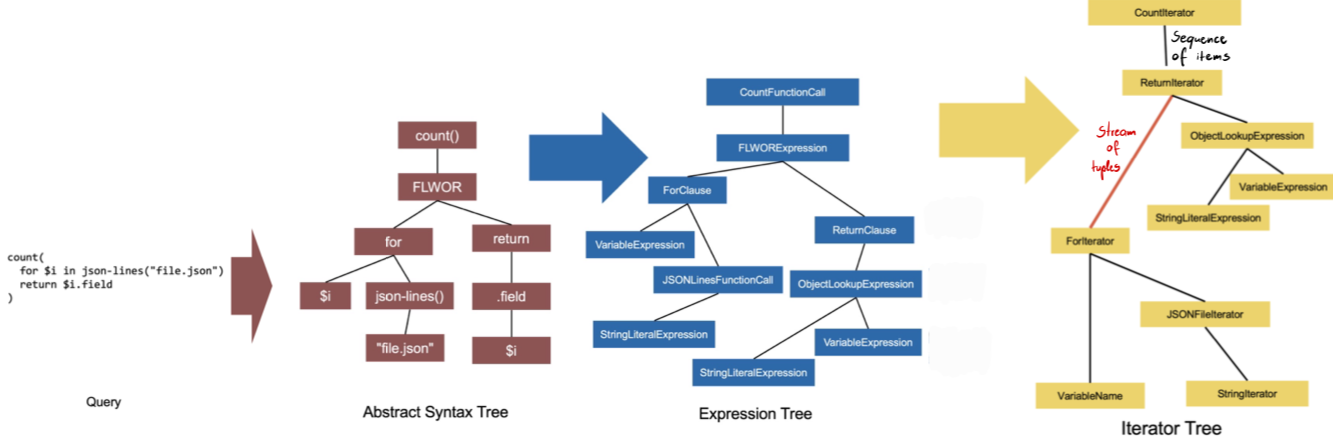
\includegraphics[width=\textwidth]{Figures/StaticPhase.png}
    \caption{Static Phase}
\end{figure}

\subsubsection{Dynamic Phase}
During the dynamic phase, the root of the tree is asked to produce a sequence of items, which is to be the final output of the query as a whole.

Then, recursively, each node in the tree will ask its children to produce sequences of items (or tuple streams). Each node then combines the sequences of items (or tuple streams) it receives from its children in order to produce its own sequence of items according to its semantics, and pass it to its parent. That way, the data flows all the way from the bottom of the tree to its root, and the final results are obtained and presented to the user or written to persistent storage (drive or data lake).

There are many different ways for a runtime iterator to produce an output sequence of items (or tuple stream) and pass it to its parent runtime iterator in the tree:

\begin{itemize}
    \item By materializing sequences of items (or tuple streams) completely in local computer memory.
    \item By locally iterating over each item in a sequence, one after the other (or over each tuple in a tuple stream, one after the other).
    \item By working in parallel over the sequence of items, internally stored as a Spark RDD.
    \item By working in parallel over the sequence fo items (or tuple stream), internally stored as a Spark DataFrame.
    \item By natively converting the semantics of the iterator to native Spark SQL.
\end{itemize}

\paragraph{Materialization}
When a sequence of items is materialized, it means that an actual List (or Array, or Vector), native to the language of implementation (in this case Java) is stored in local memory, filled with the items. This is, of course, only possible if the sequence is small enough that it fits.

The parent runtime iterator then directly processes this List in place, in order to produce its output.
A special case is when an expression is statically known to return either zero or one item (e.g., an addition, or a logical expression), but not more. Then no List structure is needed, and a single Item can be returned via a simple method call in the language of implementation (Java).

\paragraph{Streaming}
With larger sequences of items, it becomes impracticable to materialize because the footprint in memory becomes too large, and the size of the sequences that can be manipulated is strictly limited by the total memory available.

Thus, another technique is used instead: streaming. When a sequence of items (or tuple stream) is produced and consumed in a streaming fashion, it means that the items (or tuples) are produced and consumed one by one, iteratively. But the whole sequence of items (or tuple stream) is never stored anywhere.

With this technique, it is possible to process sequences that are much larger than memory, because the actual sequence is never fully stored. However, there are two problems with this: first, it can take a lot of time to go through the entire sequence (imagine doing so with billions or trillions of items). Second, there are expressions or clauses that are not compatible with streaming (consider, for example, the group by or order by clause, which cannot be implemented without materializing their full input).

\paragraph{Parallel Execution (with RDDs)}
When a sequence becomes unreasonably large, RumbleDB switches to a parallel execution, leveraging Spark capabilities: the sequences of items are passed and processed as RDDs of Item objects. Each runtime iterator then calls Spark transformations on these RDDs to produce an output RDD, or in some cases (e.g., count()) calls a Spark action to produce a single, local, materialized Item with an action.

A Spark transformation or action often needs to be supplied with an additional function (e.g., a map function, a filter function), called a Spark UDF (for “User-Defined Function”). What RumbleDB then does is that it squeezes an entire runtime iterator subtree into a UDF, so that this subtree can be recursively evaluated on each node of the cluster, as a local execution (materialized or streaming).

For example, imagine a filter expression, with a specific predicate, on a sequence of a billion items. If the input sequence is physically available as an RDD, RumbleDB squeezes the predicate's runtime iterator tree into a UDF, and invokes the filter() transformation with this UDF, resulting in a smaller RDD that contains the filtered sequence of items. Physically, the predicate's runtime iterator tree will be evalu- ated on items, in parallel, across thousands of machines in the cluster; relative to each one of these machines, this is a local execution (local to each machine), where the predicate iterator streams over each batch.

The use of RDDs is specific to sequences of items and does not exist for tuple streams.

\paragraph{Parallel execution (with DataFrames)}

The RDD implementation supports heterogeneous sequences by leveraging the polymorphism of Item objects. However, this is not efficient in the case that Items in the same sequence happen to have a regular structure.

Thus, if the Items in a sequence are valid against a specific schema, or even against an array type or an atomic type, the underlying physical storage in memory relies on Spark DataFrames instead of RDDs. Homogeneous sequences of arrays or of atomics (e.g., a sequence of in- tegers) are physical implemented as a one-column DataFrame with the corresponding type.

Thus, there exists a mapping from JSONiq types to Spark SQL types. In the case that there is no corresponding Spark SQL type, the implementation falls back to RDDs.

To summarize, homogeneous sequences of the most common types are stored in DataFrames, and RDDs are used in all other cases.

DataFrames are also consistently used for storing tuple streams and parallelizing the execution of FLWOR clauses. In FLWOR DataFrames, every column corresponds to one FLWOR variable, which is similar to the visuals provided earlier for FLWOR expressions in this chapter. The column type can either be native if the variable type can be mapped seamlessly to a Spark SQL type. Otherwise, the column type will be binary and Items are serialized to sequences of types and deserialized back on demand.


\paragraph{Parellel execution (with Native SQL)}

In some cases (more in every release), RumbleDB is able to evaluate the query using only Spark SQL, compiling JSONiq to SQL directly instead of packing Java runtime iterators in UDFs. This leads to faster execution, because UDFs are slower than a native execution in SQL. This is because, to a SQL optimizer, UDFs are opaque and prevent automatic optimizations.

RumbleDB switches seamless between all execution modes, even within the same query, as shown on the following diagram.


\begin{figure}[ht]
    \centering
    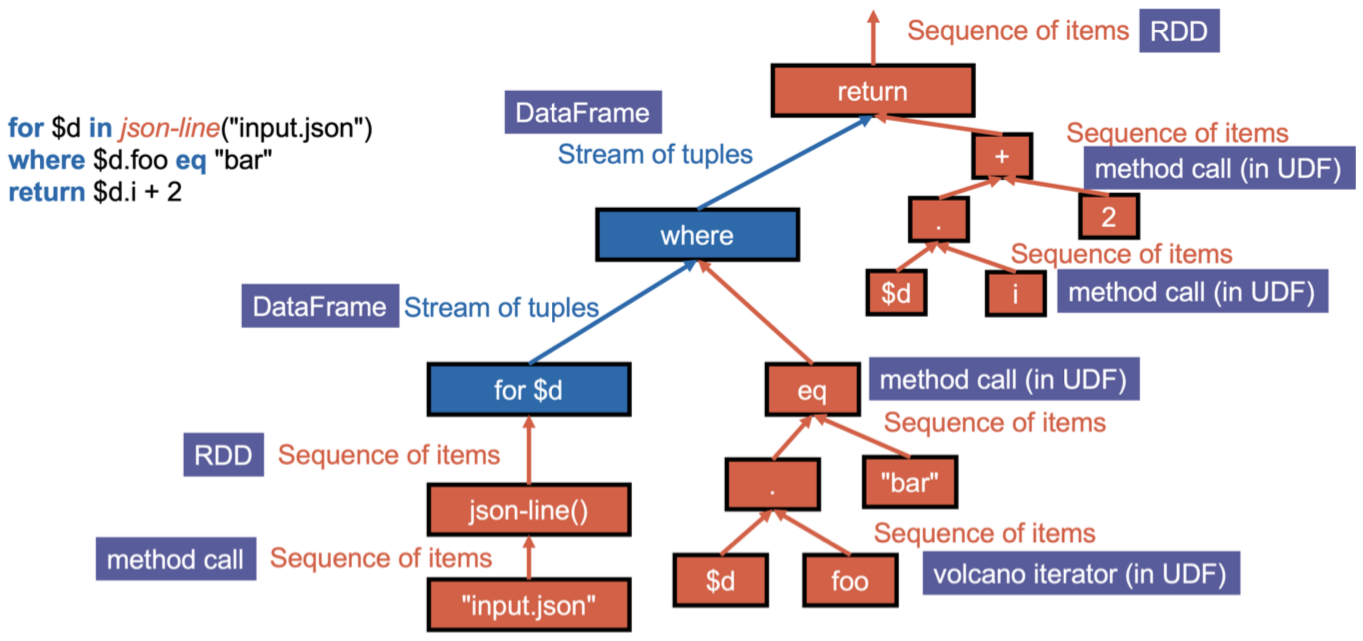
\includegraphics[width=\textwidth]{Figures/SQLExecution.png}
    \caption{Pipeline Parallel Execution with SQL}
\end{figure}



